\newcommand{\minuskb}{- k((y - u) - l_{10}) - b(\dot{y} - \dot{u})}
\newcommand{\kb}{k((y - u) - l_{10}) + b(\dot{y} - \dot{u})}

\section{Vypracování}

\subsection{Sestavení modelů}

\subsubsection{Sestavení modelu pomocí SimMechanics}

Model pomocí modulu Simulinku, první generace \textit{SimMechanics}, jsem sestavil následovně. 

\begin{figure}[htbp]
	\centering
	\includegraphics[width=0.9\textwidth]{img/simscape_1st.png}
	\caption{Model v SimMechanics}
\end{figure}
\FloatBarrier

K takovému modelu mě vedla představa zjednodušující zadaný model na následující schéma.

\begin{figure}[htbp]
	\centering
	\includegraphics[width=0.6\textwidth]{img/simplified-model.eps}
	\caption{Zjednodušení představy zadaného problému}
\end{figure}
\FloatBarrier

% Skupina \textit{World Frame} představuje \enquote{zem}, ke které je soustava vztažená. Blok \textit{Rigid Transform} otočí souřadnicový systém tak, abych se po simulaci mohl podívat na vizualizaci problému natočené ve směru osy \textit{+X}. Dalším blokem je první \textit{Prismatic Joint}. Tento blok přidává stupeň volnosti k tělesu s ním svázaným. S jeho pomocí umístím těleso do \textit{nuly}, umožním stanovit sílu, kterou je na těleso působeno, a vyvedu výstupy polohy a rychlosti. Na tento blok dále umístím těleso, jehož hmotnost nastavím na \textit{M} a pro výpočty ho \enquote{přeměním} na \textit{hmotný bod}. Na tuto skupinu umístím další \textit{Prismatic Joint} vytvářející stupeň volnosti pro druhý hmotný bod. Tento \textit{Prismatic Joint} ale těleso umisťuje do počátečního natažení pružiny a sám o sobě zavádí soustavu \textit{pružina-tlumič} o klidové délce \( l_{10} \).

Po odsimulování modelu s nastavenou počáteční podmínkou (pružina natažená na dvojnásobek své délky) získávám následující graf.

\begin{figure}[htbp]
	\centering
	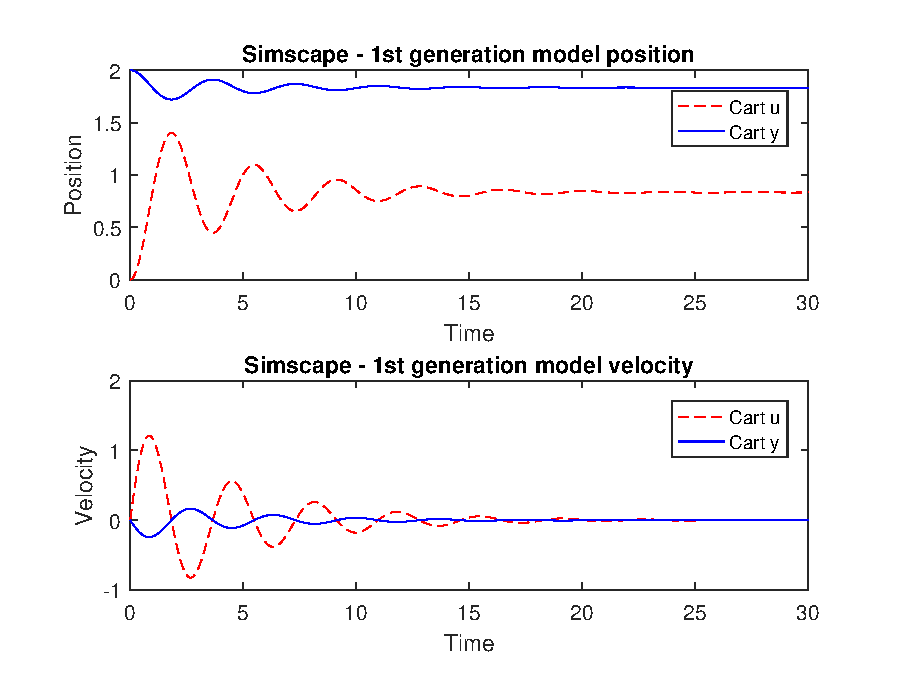
\includegraphics[scale=0.7]{graphs/simscape1.eps}
	\caption{Odsimulovaný model v SimMechanics s nenulovou počáteční podmínkou}
\end{figure}
\FloatBarrier

\subsubsection{Odvození modelu pomocí diferenciálních rovnic}

V této sekci odvodím matematický model za pomocí diferenciálních rovnic, tzv. Newton-Eulerovou metodou. V zadání je souřadnice vozíku o hmotnosti \textit{m} označena jako \textit{y}. Absolutní poloha druhého vozíku o hmotnosti \textit{M} je znázorněna proměnnou \textit{u}. Určeme si dvě síly: \( F_E \) a \( F_m \), kde \( F_E \) je síla vnější působící na spodní vozík a \( F_m \) je síla, kterou působí horní vozík na spodní. Z Newtonova zákona známe vztah pro sílu \( F = m \cdot a \). Z tohoto vyplývá, že součet síly externí a síly \( F_m \) musí být roven hmotnosti spodního vozíku vynásobené jeho zrychlením.

\begin{equation} \label{eq:1}
   F_E + F_m = M \ddot{u} 
\end{equation}

Síla \( F_m \) je dána součtem sil pružiny a tlumiče, spojující obě tělesa. Síla pružiny je určena tuhostí pružiny \textit{k} závisející na momentální délce pružiny. Momentální délka pružiny je rovna klidové délce pružiny \( l_{10} \) odečtené od rozdílu poloh těles. Síla tlumiče není závislá na rozdíl od pružiny na vlastní délce, nýbrž na rozdílu rychlostí těles takovým tlumičem spojených.

\begin{equation} \label{eq:2}
    F_m = \kb
\end{equation}

Rovnici \ref{eq:2} lze dosadit do \ref{eq:1}, z čehož vzniká rovnice \ref{eq:3}. Jelikož platí zákon akce a reakce, tak na horní vozík působí síla opačného směru, než je ta, kterou horní vozík působí na spodní a můžeme napsat rovnici~\ref{eq:4}.

\begin{align}
    F_E + \kb &= M \ddot{u} \label{eq:3} \\
    - F_m = \minuskb &= m \ddot{y} \label{eq:4}
\end{align}

Pro snazší vytváření modelu v modulu Simulink stačí vyjádřit nejvyšší derivace, které se v rovnicích vyskytují. V našem případě je taková úprava triviální.

\begin{align*}
    \ddot{u} &= \dfrac{1}{M} ( F_E + \kb ) \\
    \ddot{y} &= \dfrac{1}{m} ( \minuskb )
\end{align*}

Graf ukazuje výsledek simulace systému s počáteční podmínkou, kdy natažení pružiny je rovno dvojnásobku vlastní klidové délky.

\begin{figure}[htbp]
	\centering
	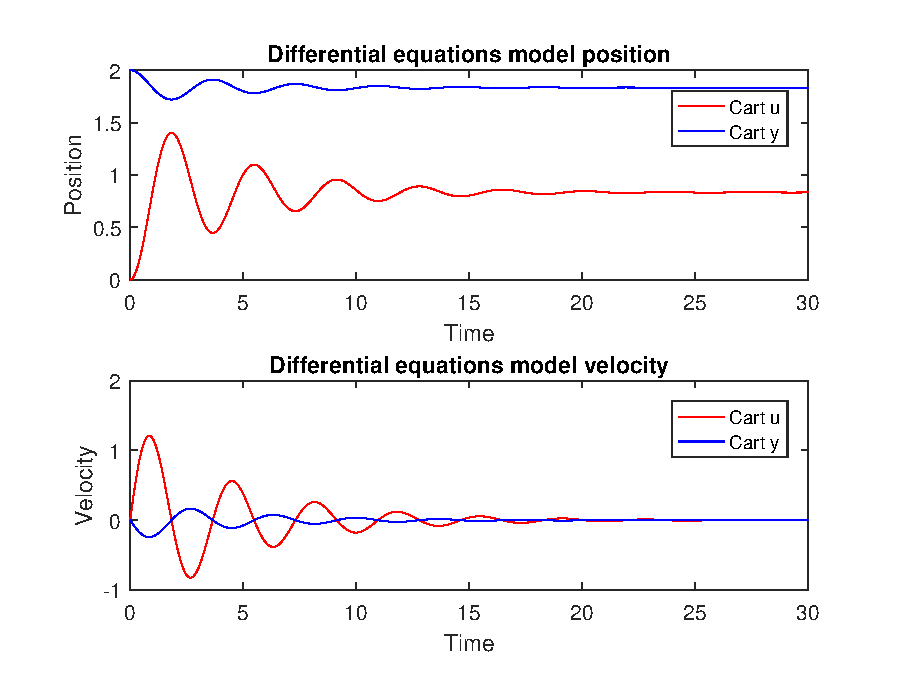
\includegraphics[scale=0.7]{graphs/equations.eps}
	\caption{Odsimulovaný model v Simulinku s nenulovou počáteční podmínkou}
\end{figure}
\FloatBarrier

\subsubsection{Linearizovaný model}

Abychom mohli v MATLABu vytvořit schéma pomocí bloku \textit{StateSpace}, musíme model nejdříve zlinearizovat.

Linearizace se provádí vždy v bodě reprezentující rovnovážný stav. V našem případě je to bod \( x(0) \).

\[ x(0) = \begin{bmatrix} u & \dot{u} & y & \dot{y} \end{bmatrix} = \begin{bmatrix} 0 & 0 & l_{10} & 0 \end{bmatrix} \]

Jako první vytvoříme stavový popis, musíme tedy zavést stavové proměnné. Ty volíme libovolně. Při tomto procesu rovnou určíme časové derivace stavových proměnných.

\noindent
\begin{minipage}[t]{.5\textwidth}
    \begin{align*}
        x_1 &= u \\
        x_2 &= \dot{u} \\
        x_3 &= y \\
        x_4 &= \dot{y} \\
    \end{align*}
\end{minipage}%
\begin{minipage}[t]{.5\textwidth}
    \begin{align*}
        \dot{x}_1 &= u \\
        \dot{x}_2 &= \dfrac{1}{M} ( F_E + \kb ) \\
        \dot{x}_3 &= y \\
        \dot{x}_4 &= \dfrac{1}{m} ( \minuskb ) \\
    \end{align*}
\end{minipage}

Nyní lze vypočítat matice \textbf{A}, \textbf{B}, \textbf{C} a \textbf{D}. Matice \textbf{A} je maticí dynamiky systému. \textbf{B} definuje, jak vstup ovlivňuje stavy systému. \textbf{C} je matice výstupu, která říká co je výstupem ze systému. \textbf{D} umožňuje, aby systémový vstup přímo ovlivňoval výstup systému. Pro většinu systémů, které jsme během kurzu uvažovali, je matice \textbf{D} nulovou maticí.

Pro snazší derivování si zjednodušme nejsložitější výrazy, tedy \( \dot{x}_2 \) a \( \dot{x}_4 \).

\begin{align*}
    \dot{x}_2   &= F_E \dfrac{1}{M} + \dfrac{k}{M} (x_3 - x_1 - l_{10}) + \dfrac{b}{M} (x_4 - x_2) \\
                &= - x_1 \dfrac{k}{M} - x_2 \dfrac{b}{M} + x_3 \dfrac{k}{M} + x_4 \dfrac{b}{M} + F_E \dfrac{1}{M} - l_{10} \dfrac{k}{M} \\
    \dot{x}_4   &= - \dfrac{k}{m} (x_3 - x_1 - l_{10}) - \dfrac{b}{m} (x_4 - x_2) \\
                &= x_1 \dfrac{k}{m} + x_2 \dfrac{b}{m} - x_3 \dfrac{k}{m} - x_4 \dfrac{b}{m} + l_{10} \dfrac{k}{m}
\end{align*}

Matici \textbf{A} získáme tak, že postupně všechny stavové proměnné derivované podle času zderivujeme parciálně podle všech nederivovaných stavových proměnných. Pro získání matice \textbf{B} pak derivujeme ne stavovými proměnnými, nýbrž vstupem systému. \textbf{C} je vektor stavových proměnných parciálně derivovaný každou ze stavových proměnných. Nakonec \textbf{D} je vektor stavových proměnných derivovaný vstupem.

\begin{align*}
    \begin{bmatrix} \dot{x}_1(t)\\ \dot{x}_2(t)\\ \dot{x}_3(t)\\ \dot{x}_4(t) \end{bmatrix} =
    \begin{bmatrix} 0 & 1 & 0 & 0\\ - \dfrac{k}{M} & - \dfrac{b}{M} & \dfrac{k}{M} & \dfrac{b}{M}\\ 0 & 0 & 0 & 1\\ \dfrac{k}{m} & \dfrac{b}{m} & - \dfrac{k}{m} & - \dfrac{b}{m}\end{bmatrix} \cdot 
    \begin{bmatrix} x_1(t)\\ x_2(t)\\ x_3(t)\\ x_4(t) \end{bmatrix} +
    \begin{bmatrix} 0\\ \dfrac{1}{M}\\ 0\\ 0 \end{bmatrix} F_E
\end{align*}

\begin{align*}
    y(t) =
    \begin{bmatrix} 1 & 0 & 0 & 0\\ 0 & 1 & 0 & 0\\ 0 & 0 & 1 & 0\\ 0 & 0 & 0 & 1 \end{bmatrix} \cdot 
    \begin{bmatrix} x_1(t)\\ x_2(t)\\ x_3(t)\\ x_4(t) \end{bmatrix} + 
    \begin{bmatrix} 0\\ 0\\ 0\\ 0 \end{bmatrix} u(t)
\end{align*}

Tyto matice můžeme předat jako parametr bloku \textit{StateSpace}, kterému na vstup přijde síla \( F_E \). Jelikož se při přechodu na linearizovaný model vyjadřuje systém v tzv. \textit{přírůstkových souřadnicích}, tak poloha vozíku \textit{y} je vyjádřena jako odchylka od svého rovnovážného stavu. To znamená, že aby se grafy linearizovaného modelu shodovaly se všemi ostatními, museli bychom k poloze vozíku \textit{y} přičíst bod, ve kterém proběhla linearizace, tedy přičíst číslo 1.

\subsection{Srovnání modelů}

\subsubsection{Počáteční podmínky 1: rovnovážný stav}

Porovnáním modelů odismulovaných v jejich rovnovážných stavech zjišťujeme, že jsou identické.

\begin{figure}[htbp]
	\centering
	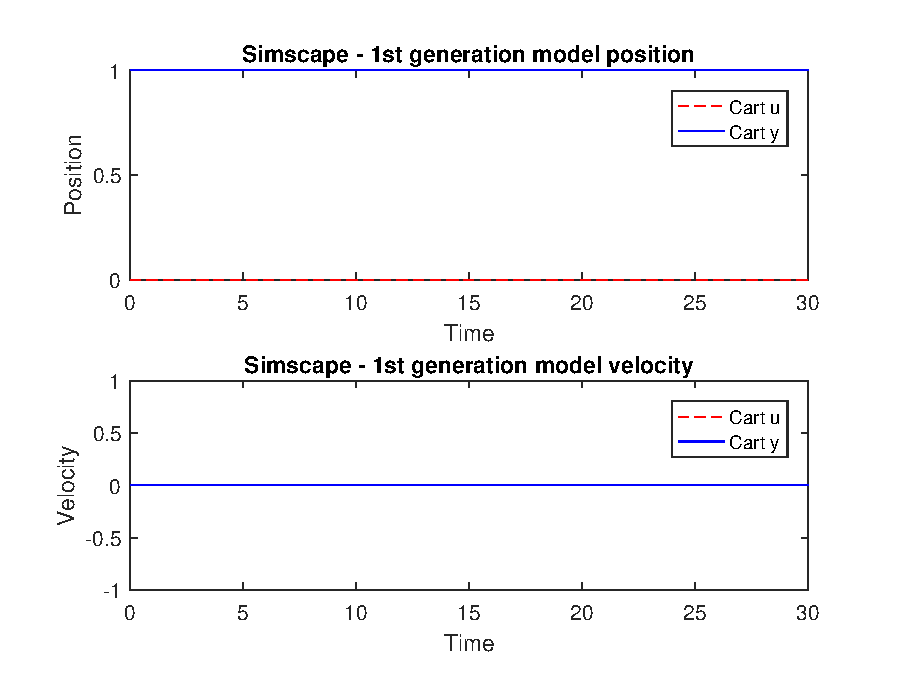
\includegraphics[scale=0.7]{graphs/simscape1_rovnovaha.eps}
	\caption{Odsimulovaný model v SimMechanics v rovnovážném stavu}
\end{figure}
\FloatBarrier

\begin{figure}[htbp]
	\centering
	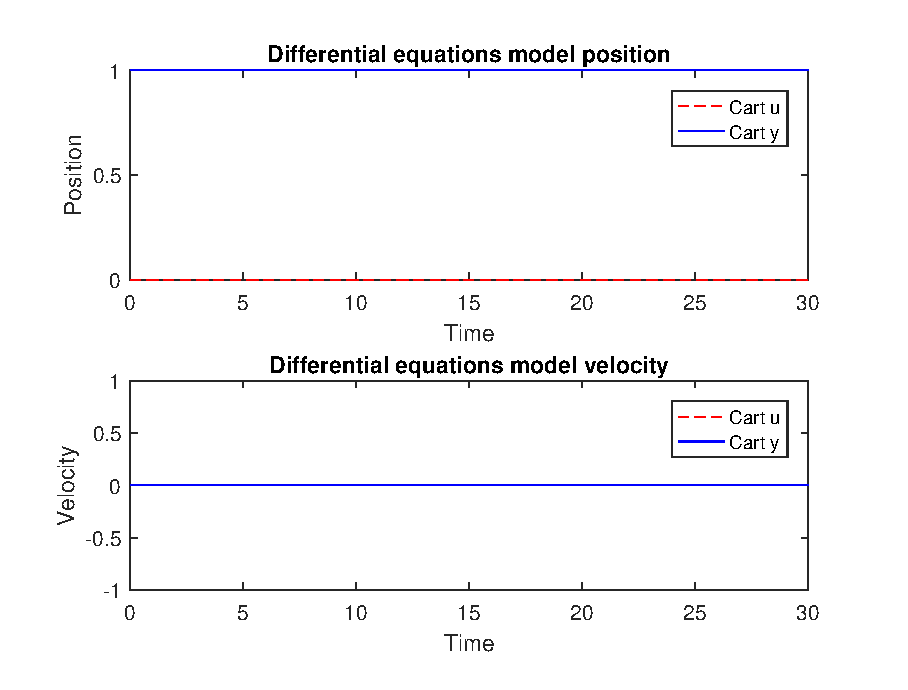
\includegraphics[scale=0.7]{graphs/differential_rovnovaha.eps}
	\caption{Odsimulovaný model diferenciálních rovnic v rovnovážném stavu}
\end{figure}
\FloatBarrier

\begin{figure}[htbp]
	\centering
	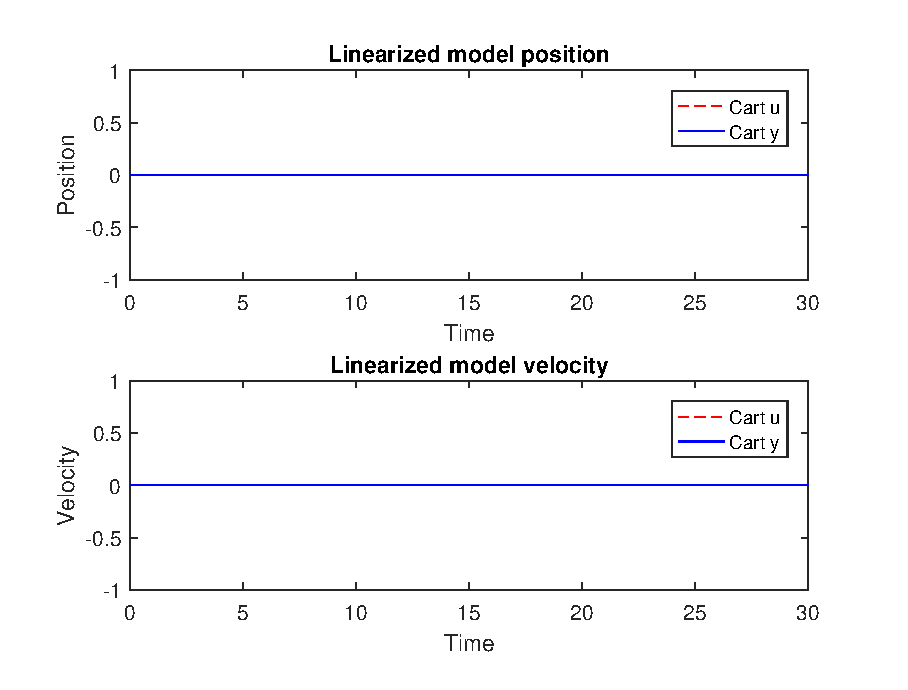
\includegraphics[scale=0.7]{graphs/linear_rovnovaha.eps}
	\caption{Odsimulovaný linearizovaný model v rovnovážném stavu}
\end{figure}
\FloatBarrier

\subsubsection{Počáteční podmínky 2: dvojnásobná délka pružiny oproti délce klidové}

Nyní, na rozdíl od předchozího případu, lze pozorovat odlišnosti modelů. Považujme graf vzniklý z diferenciálních rovnic za referenční. 

\begin{enumerate}
    \item SimMechanics: oproti referenčnímu modelu má vozík o hmotnosti \textit{m} jinou amplitudu křivky polohy i rychlosti.
    \item Linearizovaný model: oproti referenčnímu modelu je poloha vozíku o hmotnosti \textit{m} počítána od hodnoty 1 (ne od hodnoty 2 jako v referenčním modelu).
\end{enumerate}

\begin{figure}[htbp]
	\centering
	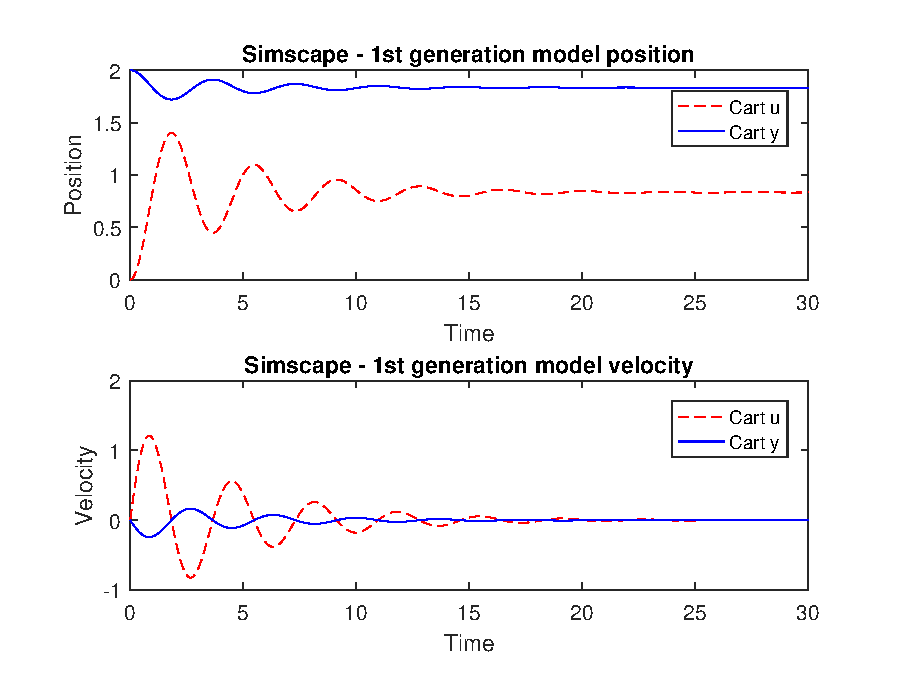
\includegraphics[scale=0.7]{graphs/simscape1.eps}
	\caption{Odsimulovaný model v SimMechanics s nenulovou počáteční podmínkou}
\end{figure}
\FloatBarrier

\begin{figure}[htbp]
	\centering
	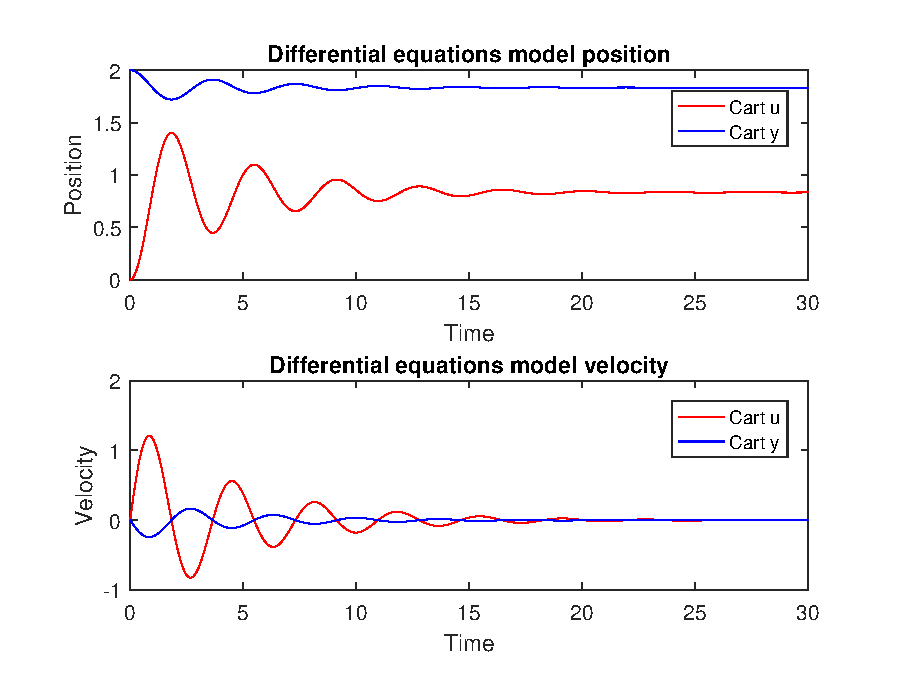
\includegraphics[scale=0.7]{graphs/equations.eps}
	\caption{Odsimulovaný model diferenciálních rovnic s nenulovou počáteční podmínkou}
\end{figure}
\FloatBarrier

\begin{figure}[htbp]
	\centering
	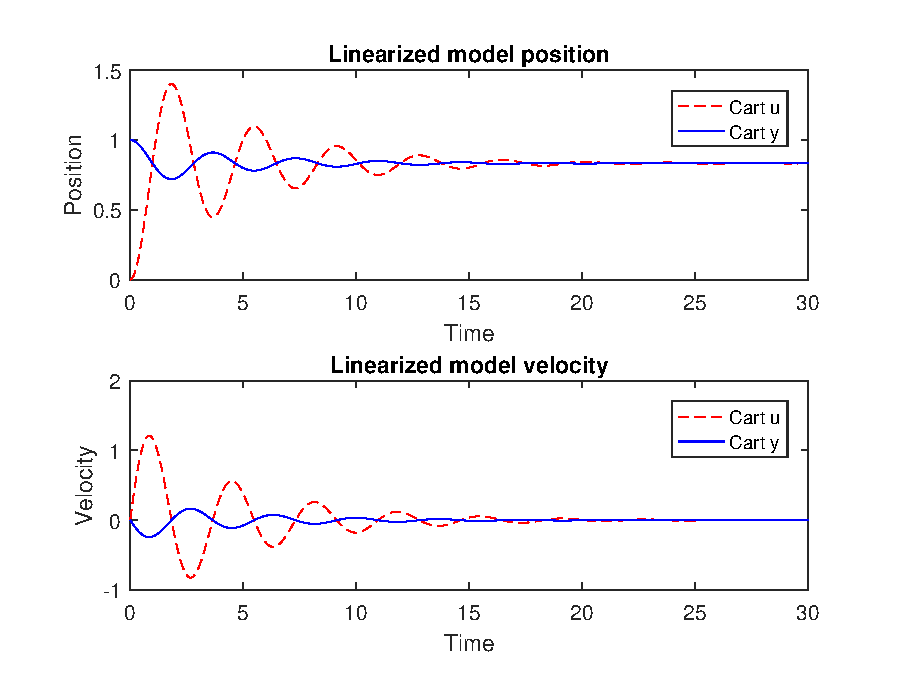
\includegraphics[scale=0.7]{graphs/linearized.eps}
	\caption{Odsimulovaný linearizovaný model s nenulovou počáteční podmínkou}
\end{figure}
\FloatBarrier

\subsection{Simulace se silou působící na soustavu}

Při působení externí síly o velikosti 10 N po dobu 10 sekund a při zanedbání tření se systém rozpohybuje v~kladném směru jedné ze souřadných os. Rychlosti vozíků se po určitém čase ustálí na stejných hodnotách a celá soustava se rozpohybuje rovnoměrným přímočarým pohybem. 

\begin{figure}[htbp]
	\centering
	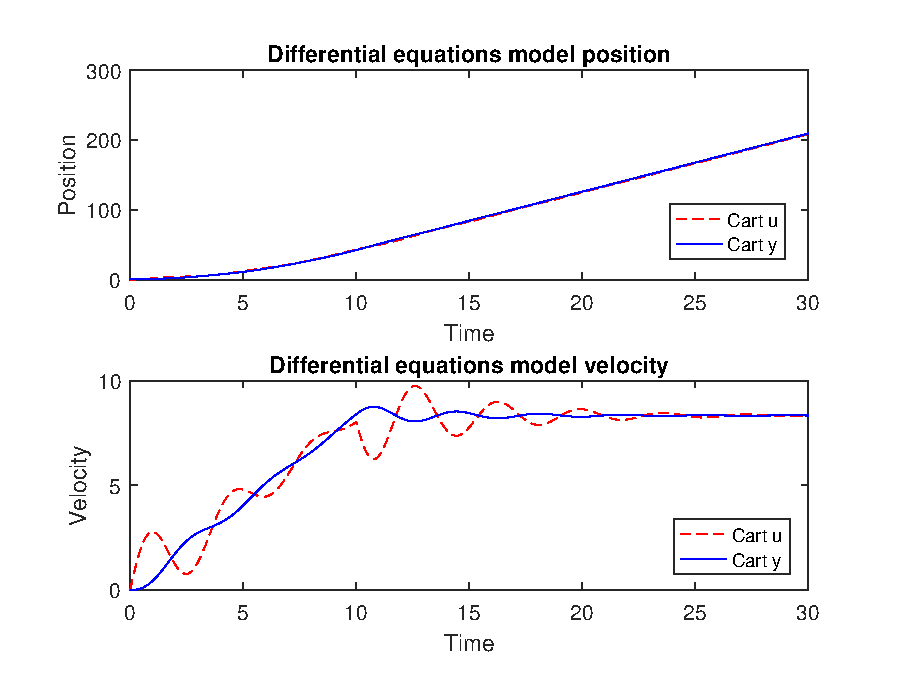
\includegraphics[scale=0.7]{graphs/differential_f10.eps}
	\caption{Chování modelu založeného na diferenciálních rovnicích s působící silou o velikosti 10 N po dobu 10 sekund}
\end{figure}
\FloatBarrier

\subsection{Frekvenční charakteristika}

K vykreslení frekvenční charakteristiky nejdříve převedeme model vyjádřený pomocí diferenciálních rovnic na přenosovou funkci. Frekvenční charakteristika je závislost zesílení na frekvenci vstupního harmonického signálu. Jako vstup máme uvažovat působící externí sílu o~velikosti 10~\textit{N} a jako výstup polohu vozíku o~hmotnosti \textit{m}.

\begin{figure}[htbp]
	\centering
	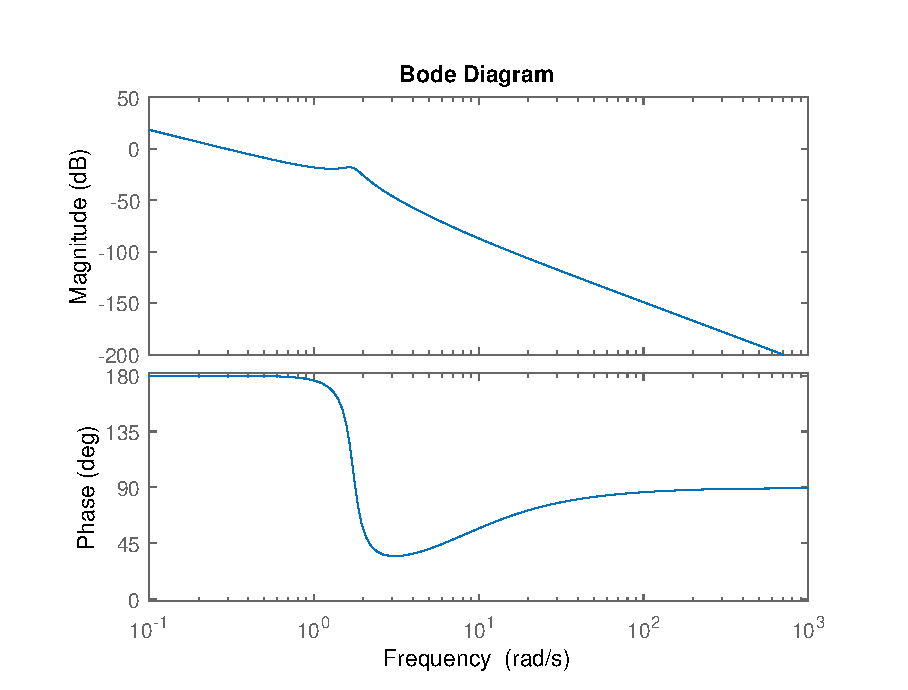
\includegraphics[scale=0.7]{graphs/bode.eps}
	\caption{Frekvenční charakteristika}
\end{figure}
\FloatBarrier

\subsection{Pozorovatelnost a nepozorovatelnost}

Pro zjištění, jestli je systém pozorovatelný, či nikoliv potřebujeme znát hodnost matice pozorovatelnosti \( O = \begin{bmatrix} C & CA & CA^2 & \ldots & CA^{n-1} \end{bmatrix}^T \), ve které je n hodnost matice \textbf{A}. Jestliže je hodnost matice pozorovatelnosti rovna hodnosti matice \textbf{A}, tak je systém pozorovatelný. 

V zadaném modelu je určení pozorovatelnosti celkem intuitivní. Jestliže budu znát polohu alespoň jednoho z vozíků, tak systém bude pozorovatelný. Jestliže budu znát jen jejich rychlost (ať už jednoho, či obou) tak nebudu schopen systém pozorovat.

V programu MATLAB určím hodnost matice \textbf{O} pomocí příkazu \texttt{rank(obsv(A, C))}.

\subsubsection{Konfigurace senzorů pozorovatelného systému}

Takto sestavená matice \textbf{C} odpovídá konfiguraci, kdy je v systému umístěn 1 senzor snímající polohu vozíku \textit{u} o hmotnosti \textit{M}. Hodnost matice \textit{O} je 4, systém je pozorovatelný.

\begin{align*}
    C = \begin{bmatrix} 1 & 0 & 0 & 0\\ 0 & 0 & 0 & 0\\ 0 & 0 & 0 & 0\\ 0 & 0 & 0 & 0 \end{bmatrix}
\end{align*}

\subsubsection{Konfigurace senzorů nepozorovatelného systému}

Takto sestavená matice \textbf{C} odpovídá konfiguraci, kdy jsou v systému umístěny 2 senzory snímající rychlosti obou vozíků. Hodnost matice \textit{O} je 3, systém je nepozorovatelný.

\begin{align*}
    C = \begin{bmatrix} 0 & 0 & 0 & 0\\ 0 & 1 & 0 & 0\\ 0 & 0 & 0 & 0\\ 0 & 0 & 0 & 1 \end{bmatrix}
\end{align*}

\section{Závěr}

V semestrální práci jsme si vyzkoušeli vytvořit několik modelů zadaného fyzikálního systému. Modely jsme porovnali a prozkoumali jeho vlastnosti. Došli jsme k závěru, že při zanedbání tření a dodání vnější energie či při nenulových počátečních rychlostech systém diverguje, vozíky se pohybují do nekonečna.
